\documentclass[pldi]{sigplanconf-pldi15}

\usepackage{url}                  % format URLs
\usepackage{listings}          % format code
\usepackage[colorlinks=true,allcolors=purple,breaklinks,draft=false]{hyperref}   % hyperlinks, including DOIs and URLs in bibliography
% known bug: http://tex.stackexchange.com/questions/1522/pdfendlink-ended-up-in-different-nesting-level-than-pdfstartlink
\newcommand{\doi}[1]{doi:~\href{http://dx.doi.org/#1}{\Hurl{#1}}}   % print a hyperlinked DOI
\usepackage{amssymb}
\usepackage{todonotes} %TODO Remove for final submission

\newcommand{\TODO}[1]{[\textsl{#1}]}
\newcommand{\code}[1]{\texttt{#1}}
\newcommand{\package}[1]{\code{#1}\cite{#1}}



\setcounter{tocdepth}{4} %TODO Remove for final submission

\begin{document}

\lstset{basicstyle=\footnotesize\ttfamily,mathescape=true,basewidth=0.5em}

\conferenceinfo{PLDI '15}{June 12---20, 2015, Portland, OR, USA.}
\copyrightyear{2015}
%\copyrightdata{}

%\titlebanner{banner above paper title}        % These are ignored unless
\preprintfooter{DRAFT - do not distribute}   % 'preprint' option specified.

\title{Efficient Multiple Dispatch in Julia}
%\subtitle{Subtitle Text, if any}

%\authorinfo{Jeff Bezanson \and Jake Bolewski \and Jiahao Chen \and Stefan Karpinski \and Jean Yang \and Alan Edelman}
%	{Massachusetts Institute of Technology}
%	{bezanson@mit.edu, jake.bolewski@gmail.com, jiahao@mit.edu, stefan@karpinski.org, jeanyang@mit.edu, edelman@mit.edu}

\maketitle

\begin{abstract}
Scientific programs are often written as software experiments operating on
code and data that have not be formally described. Such experimental software
is easier to write in dynamically typed languages. Unfortunately,
dynamic types often make it difficult to execute code efficiently. In this
paper, we describe the type system and multiple dispatch mechanism for the
Julia programming language, which is specialized for scientific computing. Julia has a
novel semantics based on efficient multiple dispatch. Julia combines
programmer-specified type tags with a type inference engine to statically
optimize method dispatch. Julia is dynamically typed in that the compiler does
not statically reject ill-typed programs, but Julia is designed to optimize
static type and dispatch inference. We describe the Julia language and type
system and our implementation of type inference and multiple dispatch
mechanisms for Julia. To demonstrate the relevance and potential impact of
designing a language based around multiple dispatch, we also describe the
manifestations of multiple dispatch in Julia's standard library.
\end{abstract}

\category{D.3.3}{PROGRAMMING LANGUAGES}{Language Constructs and Features}

\terms Languages, Multiple dispatch, Multimethods

%\keywords
%Language design, run-time system

\tableofcontents %TODO remove for final submission

\section{Dynamic languages are useful for technical computing}

\begin{quote}
	[L]a math\'ematique est l'art de donner le m\^eme nom \`a des choses
	diff\'erentes... Quand le langage a \'et\'e bien choisi, on est tout
	\'etonn\'e de voir que toutes les d\'emonstrations, faites pour un
	objet connu, s'appliqu\-ent imm\'ediatement \`a beaucoup d'objets
	nouveaux... c'est l'un des caract\`eres auxquels on reconna\^it les
	faits \`a grand rendement, ce sont ceux qui permettent ces heureuses
	innovations de langage. \cite{Poincare1908}
	
	\textit{Mathematics is the art of giving the same name to different
	things... When the language has been well chosen, one is amazed to see
	how all the statements, made for a known object, apply immediately
	to many new objects... this is one of the characteristics by which one
	recognizes high-yield facts, they are the facts which permit successful
	innovations of language.}
\end{quote}

Engineers, mathematicians and scientists routinely write software for
computational simulations and data analysis to discover new insights.
Users writing code for the purposes of discovery often by definition do not
know what computations they need upfront, but rather discover what they want by
iterating through several different prototypes. Consequently, technical
computing code is often the product of an organic process of continuous
experimentation, rather than derived from formal software engineering
specifications.

Static languages focus on being able to prove correctness of programs, and
compilers usually contain features like type checkers which constrain the set
of allowed programs in favor of provable correctness~\cite{Pierce2002}. Code written in static
languages must be able to account for all possible behaviors of the algorithms
implemented for all possible input values. All these possible code paths must
be stated at compile time, posing challenges for authors of technical codes which
often work on enormous inputs and may fail in subtle ways that require further
investigation and mitigation. Furthermore, these static analyses for
correctness tend to concern themselves with only the interface to data types,
not with their internal representation. Consequently, the formal logic of
program correctness does nothing for user concerns about performance, since
they abstract away memory layout details which are crucial for understanding the
impact of hardware factors such as bus latency and bandwidth. In contrast,
dynamic languages embody a realist philosophy: programs are not checked for
correctness, but are executed until termination or when a runtime error is
thrown. The focus is to make sense out of whatever program a user may write.
Thus dynamic languages are more permissive and expressive in ways that are more
naturally suited for rapid prototyping and experimentation.

In other words, a scientist will often run a program in order to find out what
it does---\emph{proving} anything about what it does would be premature, and an
unwelcome distraction. As a result, dynamic languages like
MATLAB~\cite{matlab}, Python~\cite{pythonlib,pythonref} and R~\cite{rlang} have
become popular amongst technical computing users for writing prototype codes.
However, code written in these languages are difficult to execute performantly;
the dynamic nature of these languages pose significant challenges for
implementers to transform code into efficiently executable
forms~\cite{Joisha2001,Joisha2006,Seljebotn2009}. Technical computing users
thus face a dilemma known as the two-language problem: it is easier to
prototype code in a dynamic language, but faster to run code written in a
static language. The two-language problem can be viewed as an unavoidable
consequence of Ousterhout's dichotomy of classifying programming languages into
scripting vs.\ system languages~\cite{Ousterhout1998,Hoare2014}. 

Julia~\footnote{Julia is free and open--source software available from
\url{http://julialang.org} under the MIT license. In this paper, we describe
the behavior of the v0.3.2 point release.} is a dynamic language designed with
the ambitious goal of eliminating the false dichotomy between dynamism and
speed~\cite{Bezanson2012,Bezanson2014b}. The language features several
different mechanisms for expressing polymorphism, namely:

\begin{itemize}
	\item A user extensible type system featuring subtyping and parametric
		types, and
	\item A user extensible generic function system with dynamic multiple
		dispatch
\end{itemize}
%
which together naturally express the polymorphism inherent in technical
computing. Julia's implementation also features a just-in-time compiler which
performs extensive static optimizations such as:

\begin{itemize}
	\item Automatic type inference, which minimizes the overhead of dynamic
		multiple dispatch and largely eliminates the need for explicit
		type annotations in function bodies,

	\item Tuple elimination,
	\item Function inlining, and
	\item Other compiler optimizations such as dead code elimination that
		are provided by the LLVM library~\cite{Lattner2004}.
\end{itemize}

This paper aims to explain how Julia's language constructs and compiler
optimizations conspire to provide expressiveness without compromising
performance, by carefully designing a language that is purposely amenable to
static analysis. When combined with an extensive base library for parallel
execution and numerical analysis, Julia provides a convenient environment for
rapid prototyping of new analytics which can also be deployed performantly,
often within a factor of two of the speed of native, hand-written C code.



\section{Type system}

Julia is a dynamic language, i.e.\ it has no static semantics. As such, Julia
does not have types in the strict sense, but rather run-time type tags used to
differentiate heap-allocated objects~\cite[Section 11.10, p. 142]{Pierce2002}.
Nevertheless, the formal theory of dynamic type tags is well defined as static
promises that are coerced at run--time into 
types~\cite{Henglein1994,Shields1998,Baars2002}, and there should be no ambiguity
in using the terms ``type'' and ``type tag'' in this paper. This
section aims to describe how dynamic type tags can be used, not for type
checking to statically reject ill-typed programs, but rather to disambiguate
objects and facilitate dispatch in ways similar to static
types~\cite{Tratt2009,Kell2014}.

All values in a dynamically typed language have two semantic components:
a \emph{tag} and some \emph{data}. The tag classifies the data, which are the
contents of some block of memory whose format is set by the programming
language. Tags are useful for both users and compilers for deciding what to do
to values, but incur overhead which increases the memory footprint of a data
item. This overhead motivates most dynamically typed languages to simplify and
minimize their tag systems.

In contrast, Julia's types are designed for expressiveness, resulting in fewer
components to the language design. An important example is arrays, which are
special cased in some languages for performance reasons, but in Julia are
described as a particular kind of parametric type, with the type parameter
encoding information about memory layout.~\cite{Bezanson2014}. In general,
Julia's types allow programs to reason about:

\begin{itemize}
\item when code is applicable (dispatch),
\item what to specialize on,
\item memory layout, and
\item what can be statically known about a potential value.
\end{itemize}
%
Furthermore, types are first-class values, allowing programs that can compute
on types and reason about all of the above.


\subsection{Kinds of types}

Julia has different kinds of types which can be formally summarized as:

\begin{lstlisting}
Type ::= Abstract | Data | Tuple | ForAll | Union | Singleton
Abstract ::= Name (P) Super }
Data ::= Name (P) Super Repr } invariant, nominative
Tuple ::= (T1, T2, ...) | (T1, T2, ..., Tn, ...) } covariant
ForAll ::= $\forall$ (lb <: T <: ub) . Type
Union ::= U (T1, T2, ...)
Singleton ::= Lift Value
TypeVar ::= lb <: Name <: ub

Tag ::= Data | Tuple
\end{lstlisting}

\begin{description}

\item[Data constructor/Tag types] are types with associated constructors. They
	are further subdivided into:
	\begin{description}
	
	\item[Bits types] like double precision floating point numbers
	(\verb|Float64|) and 32-bit signed integers (\verb|Int32|), which can
	be stored unboxed as raw bits without tag overhead,

	\item[Abstract data types] which have an internal representation
		declared with the \verb|type| keyword, and
		
	\item[Immutable types] which are similar to abstract data types
		declared with the \verb|immutable| keyword, but whose internal
		variables are immutable, thus potentially allowing for unboxed
		representations.

	\end{description}


\item[Tuple types] \code{(T1, T2,...)} which are constructed from the Cartesian
	product of zero or more existing types \code{T1}, \code{T2},
	etc.~\cite[Sec. 11.7]{Pierce2002} Tuples are covariant.

\item[Abstract types] define an uninstantiable type with no declared
	representation. They are used as declared supertypes of leaf types
	(which are concrete and instantiable).

\item[Singleton types] are constructed with the \code{::Type\{T\}} syntax and
	are used  primarily for computations on types themselves, such as
	type promotions, and for dispatch.

\item[Union types] declared as \code{Union(T1, T2,...)} are the join of zero,
	or two or more, types \code{T1}, \code{T2}, ...~\cite[Sec.
	15.7]{Pierce2002}
	%
	\begin{equation}
		\texttt{Union}(T_1, T_2, ..., T_N) = \bigvee_{i=1}^N T_i 
	\end{equation}
	%
	The union with zero types, \code{Union()}, is simply the bottom type.
	%
	Julia's \code{Union}s are untagged and disjoint, which allows for some
	simplifications in their construction:
	\begin{itemize}
		\item If there are types \code{S} and \code{T} obeying the
			subtyping relation \code{S <: T} in the union
			constructor, then \code{S} is deleted ($\beta$-reduced)
			from the final union type constructed. This
			simplification includes the special case where \code{S}
			and \code T are identical.

		\item A union type \code{Union(T)} with a single type parameter
			\code{T} is identical (by $\eta$-reduction) to just
			\code{T}.
	\end{itemize}

\item[\code{TypeVar}s] are not types, but are quantifications over sets of
	types. They are used to define constraints on type parameters in type
	constructors, and also
	
\item[\code{ForAll} types] which quantify over all types between a lower bound
	and upper bound.

\end{description}

The usefulness of types is further augmented by polymorphic features like type
parameters and subtyping, which when combined with the late binding associated
with dynamic dispatch, facilitates code reuse and an incremental style of
programming~\cite{Castagna1997} that is well--suited to the rapid prototyping
of technical codes.

\paragraph{Subtyping} Julia requires every type other than $\top$ and $\bot$ to
have exactly one declared supertype (defaulting to $\top$ if not explicitly
declared). The consequences are threefold:

\begin{itemize}

	\item Julia supports strong behavioral subtyping~\cite{Liskov1994}:
		objects of a given type can be replaced with objects of their
		subtype without altering desirable program behavior. In other
		words, subtypes obey the Liskov substitution
		principle~\cite{Liskov1974}.

	\item The subtype relation \verb|<:| defines a partial ordering on types,
		which together with the meet operation ($\wedge$) constructing
		type intersections and the join operation ($\vee$) constructing
		type unions, provide the mathematical structure needed to
		define a lattice of types~\cite{Scott1976}. Furthermore, the 
		presence of the top ($\top$, \verb|Any|) and bottom ($\bot$,
		\verb|Union()|) types means that the lattice is complete, which
		has important consequences for the ability to define data flow
		type inference algorithms~\cite{Kam1977,Khedker2009}.

	\item Julia does not support multiple inheritance, which thus far has
		not significantly decreased the usefulness of the type system.

\end{itemize}

The notion of subtyping is analogous to subset relations, but the subset
relation is not just over sets of permitted values, but also the interface,
i.e.\ set of functions allowed to compute over the types being
compares~\cite{Scott1976,Liskov1974,Liskov1992}. Furthermore, a mathematical
quantity can have more than one encoding as a compiler value. For example, each
integer in the set {0, 1, \dots, 255} has a 1:1 correspondence with an 8-bit
unsigned integer (\verb|Uint8|), and also a 1:1 correspondence as a
double-precision floating point number (\verb|Float64|). Nevertheless,
\verb|Uint8| is \textit{not} a subtype of \verb|Float64| since not all
operations on the former behave identically to operations on the latter. One
example is subtraction, which returns different values for the different types:

\begin{lstlisting}
julia> uint(5)-uint(253)
0xffffffffffffff08

julia> 5.0 - 253.0
-248.0
\end{lstlisting}
%
In contrast, \verb|Union(Uint8, Float64)| is a subtype of \verb|Real| by
transitivity of the declared supertype relations, which allow \verb|Real|
to abstractly represent disjoint sets of values and their interfaces.


\subsection{Type parameters}

Julia types can also take one or more parameters which are also types. Such
parametric polymorphism is akin to a dynamic form of C++ template
specialization.

A parametric type is defined as a type with additional parameters specified
within braces, e.g.:

\begin{lstlisting}
abstract foo{S, T<:Real, Int<:U<:Signed}
\end{lstlisting}
%
\verb|foo| is defined with three \verb|TypeVar|s which act as placeholders for
types. \verb|T| and \verb|U| are bounded \verb|TypeVar|s, which constrain the
set of allowed types which can be placed in their respective slots. For
convenience, an unbound type parameter can be omitted from a parametric type
declaration. For example, \verb|Array| is a synonym for \verb|Array{T, N}|
for some unspecified element type \verb|T| and rank \verb|N|, and is convenient
shorthand for writing methods that are agnostic about these type parameters.

The subtyping rules for parametric types require reasoning about variance,
i.e.\ the relation between subtype relations of the parametric types and
subtype relations of the parameters. The conventional wisdom is that type
safety allows covariance if components are read but not written, and
contravariance if they are written but not read~\cite{Castagna1995}. As type
parameters can represent the types of mutable fields in a \verb|type| which can
be read or written, then the only safe choice is invariance. Thus Julia's
parametric types are invariant.

Parametric invariance has some subtle consequences for Julia's type system.
First, parametric types introduce many short, finite length chains into the
type lattice. Consider the very simple type system of
Figure~\ref{fig:lattice}a, with two leaf (instantiable types) types \textbf{1}
and \textbf{2} representing singleton values 1 and 2 of the natural numbers,
\verb|Nat|. A user can augment the lattice with a new parametric type
\verb|S{T}|. If there is no restriction whatsoever on the type parameter
\verb|T|, then there are 5 different parametric types of the form \verb|S{T}|.
Furthermore, each \verb|S{T}| has supertype \verb|S| by construction, and by
invariance of \verb|T| there are no values of the type parameters \verb|T| and
\verb|U| such that \verb|S{T}| is a subtype of \verb|S{U}|. Additionally, none
of the types \verb|S{T}| is a subtype or supertype of any of \textbf{1},
\textbf{2} or \verb|Nat|. Thus each \verb|S{T}| appears in exactly one finite
poset $\bot$ \verb|<: S{T} <: S <:| $\top$, and the new type lattice has the
structure shown in Figure~\ref{fig:lattice}b. Note that \verb|S{|$\top$\verb|}|
is a concrete type with type parameter $\top$ (\verb|Any|), while \verb|S{T}|
is a synonym for the abstract type \verb|S| where \verb|T| is a \verb|TypeVar|
with lower bound $\bot$ and upper bound $\top$. 

\begin{figure}
	\centering
	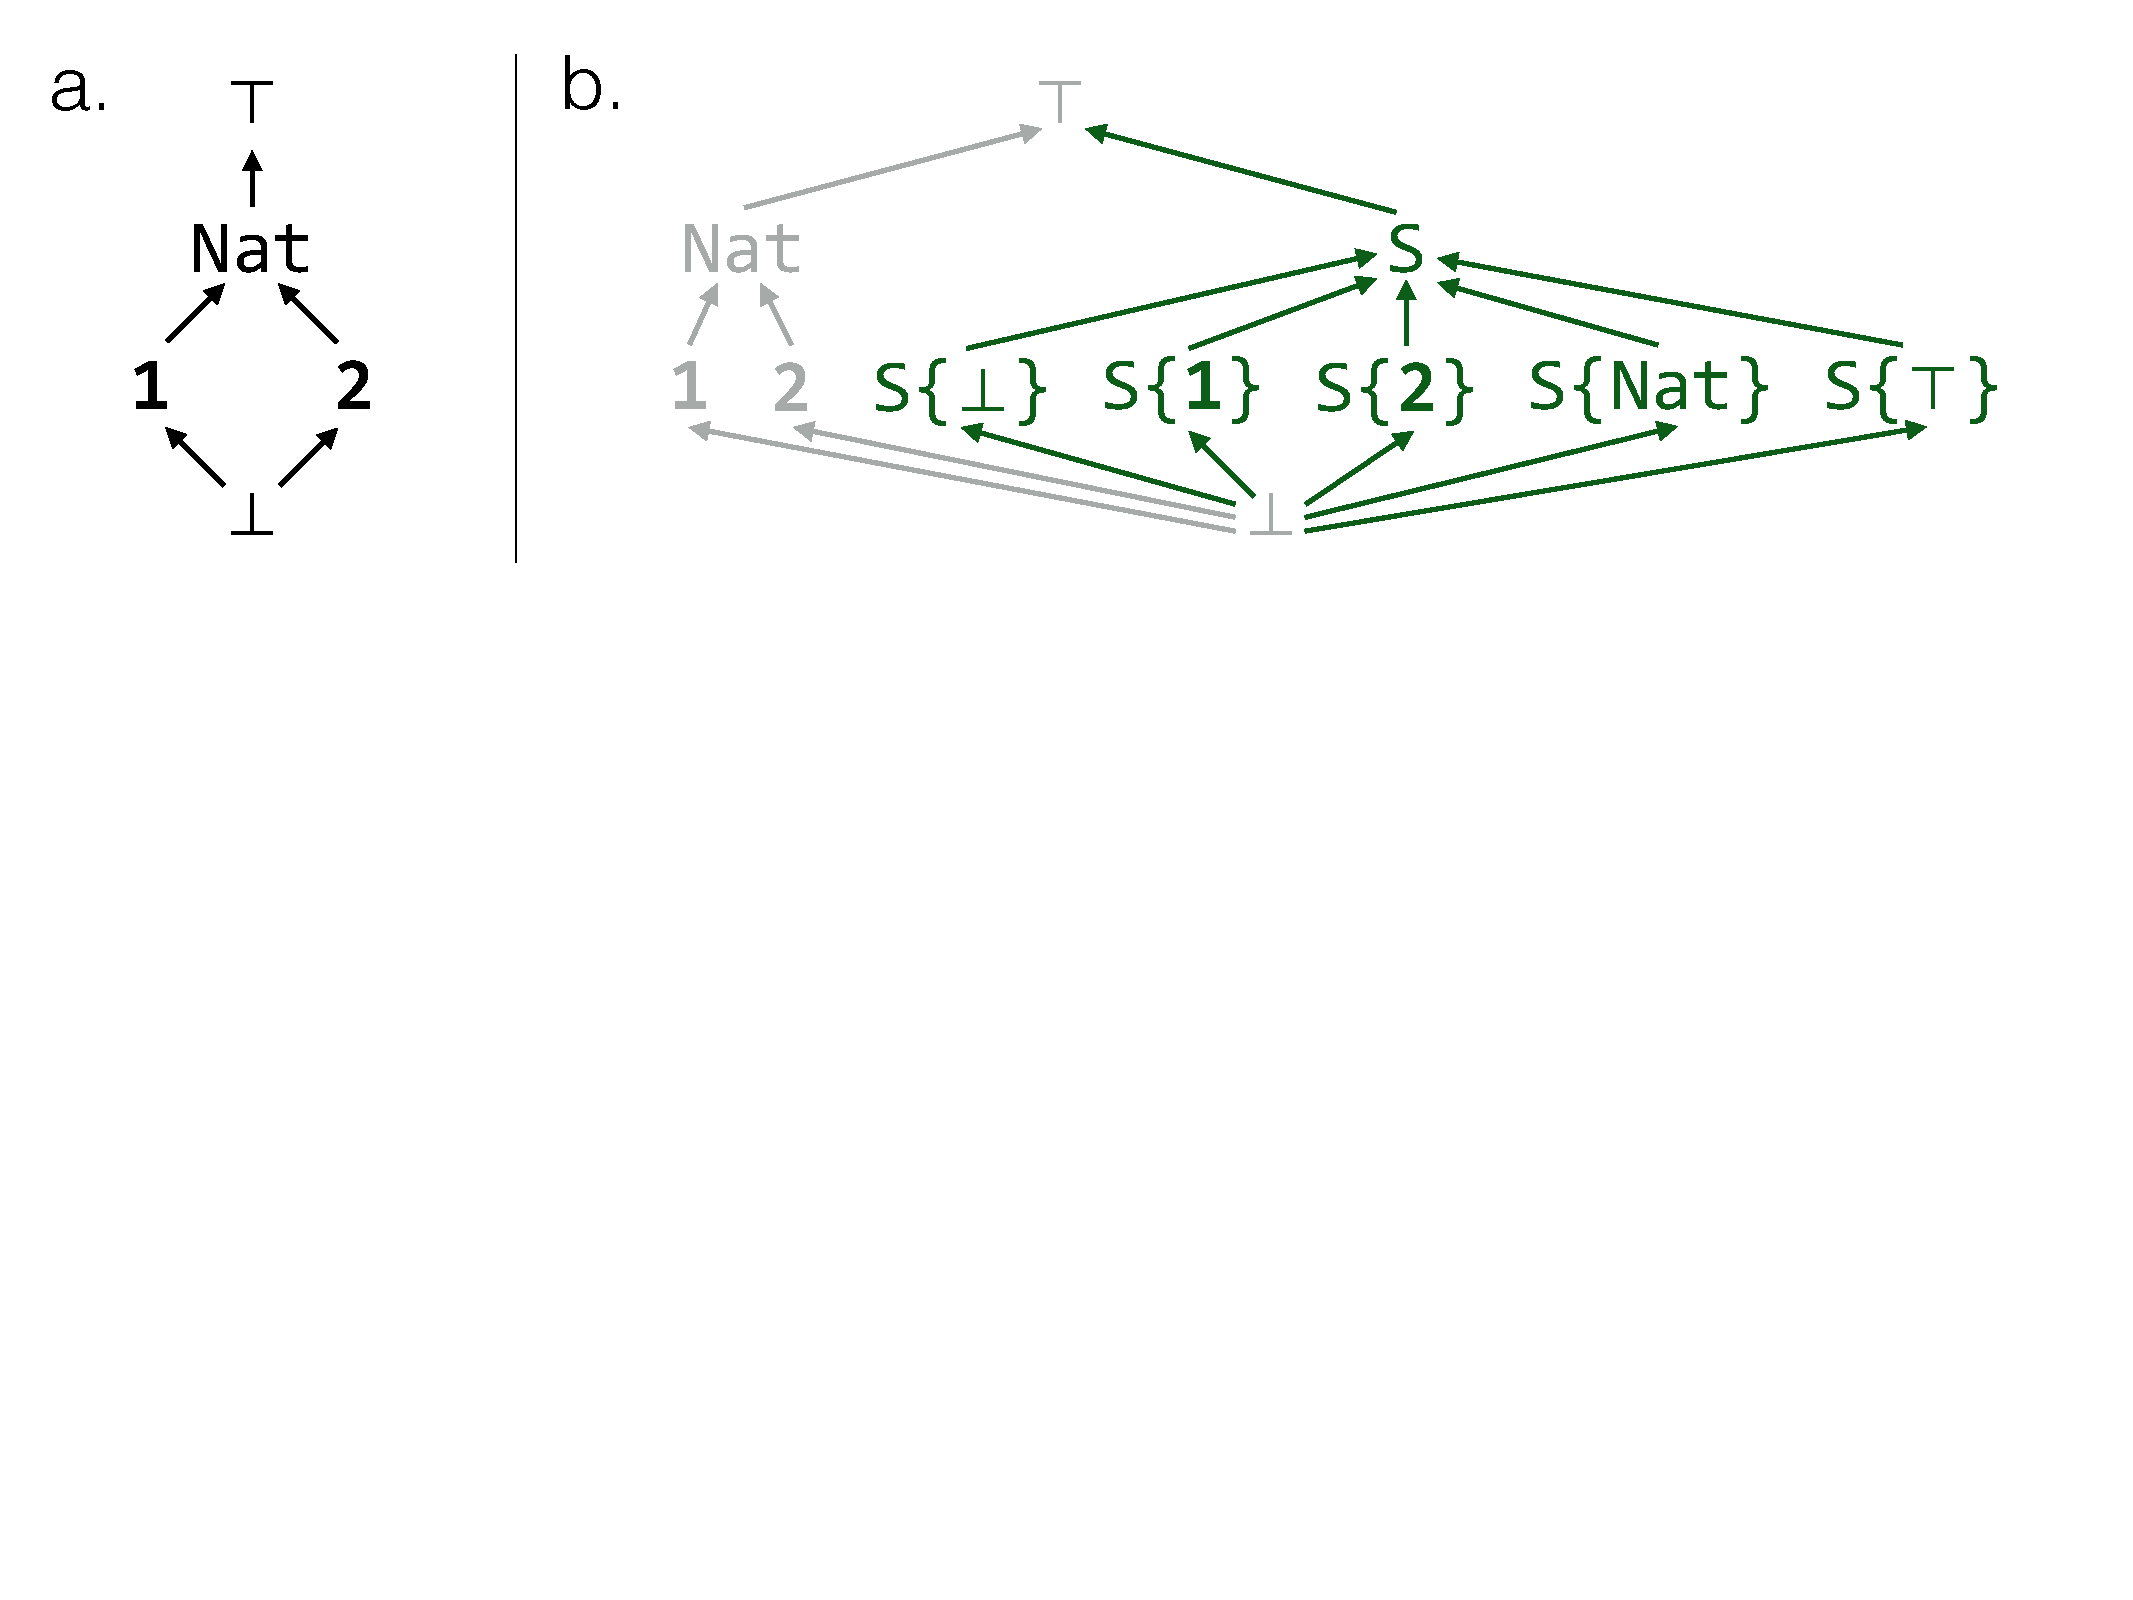
\includegraphics[width=\columnwidth]{fig-lattice}
	\caption{
		\textbf{a.} A simple lattice with bottom type $\bot$, top type
		$\top$, singleton types \textbf{1} and \textbf{2}, and their
		supertype \texttt{Nat}.
		\textbf{b.} The same lattice extended with a parametric type
		\texttt{S\{T\}} with no restriction on the type parameter
		\texttt{T}, showing that for each \texttt{T}, invariance
		requires that the corresponding type \texttt{S\{T\}} be a leaf
		type (i.e.\ instantiable), even if \texttt{T} itself is not a
		leaf type.}
	\label{fig:lattice}
\end{figure}

Second, the example of Figure~\ref{fig:lattice} illustrates how invariance of
type parameters requires parametric types to be instantiable with any type
parameter, regardless of whether the parameter corresponds to an abstract or
concrete type. The rationale for this behavior allows for the Julia compiler to
reason about different representations, and is perhaps best explained in the
context of arrays. For arrays, the type parameter describes the set of possible
element types ~\cite{Bezanson2014}, so an \verb|Array{Float64}|
can only contain concrete elements of type \verb|Float64|, whereas an
\verb|Array{Real}| can contain elements that are subtypes of \verb|Real| such
as \verb|Int|, \verb|Float64| or even \verb|Rational|. The former array
consists of concrete immutable elements and can be reified with a single
pointer to a contiguous memory block with the tags for each element elided,
resulting in a memory layout which can interoperate with C or Fortran code as
native array data structures. The latter array can store more diverse objects,
but the element type provides no information about the mutability of each
element. Consequently, the array must be represented in memory with pointers to
boxed elements, so that checks from generated LLVM code can be inserted that
call back into the Julia runtime to determine the actual type of the stored
element at run--time. Thus describing arrays as parametric types allows
different data structures to be used under the hood without any semantic
changes imposed on users, thus allowing for more performance in one case and
greater flexibility in the other.

Subtyping and type parameters combine to provide powerful expressions of
polymorphism, as formalized by $\lambda$--calculi such as
System~F$_\le$~\cite{Cardelli1985}. However, the interaction of these two
Julia languages features can be subtle and confusing. For example, \verb|Real|
is not a subtype of \verb|Complex| because for each type \verb|T| that is a
subtype of \verb|Real|, there is a corresponding instantiable type
\verb|Complex{T}|. None of these correspond to \verb|Real| since there is no
\verb|T| such that \verb|Complex{T}| is a one-component number, and each
concrete type only has $\bot$ as its subtype.

Another more subtle situation arises from parametric invariance: each value of
\verb|Complex{Int64}| is a Gaussian integer, i.e., a complex number where each
component is an integer, and so each \verb|Complex{Int64}| is in 1:1
correspondence with a value in \verb|Complex{Integer}| and also in
\verb|Complex{Real}|. Nevertheless, \verb|Complex{Int64}| is a subtype of
neither \verb|Complex{Integer}| nor \verb|Complex{Real}| due to parametric
invariance. However, all of these are subtypes of \verb|Complex|.


\subsection{Type conversion}

\TODO{Explain type conversion}


\subsection{Type promotion}

Type promotions are written as user-level code to compute new types.

\TODO{Explain type promotion}


\subsection{Example: complex numbers}

Example: the \code{Complex} type defined by

\begin{lstlisting}
immutable Complex{T<:Real} <: Number
    re :: T
    im :: T
end
\end{lstlisting}
%
has two declared fields, \code{re} and \code{im}. Each of these fields has the
type annotation \code{::T}. The type parameter \code{T} is constrained to be a
subtype of \code{Real}, and \code{Complex} itself has a declared supertype
which is \code{Number}.

\code{Complex} comes with a default, implicitly defined inner constructor

\begin{lstlisting}
Complex{T<:Number}(re::T, im::T) = new(re, im)
\end{lstlisting}
%
which makes use of a special intrinsic function \code{new} to allocate new
memory for the fields \code{re} and \code{im}. Inner constructors can be
defined by the user, in which case the default inner constructor is not
generated.

An instance of \code{Complex} can be created using the inner constructor, e.g.\

\begin{lstlisting}
z = Complex{Float64}(0.0, 1.0)
\end{lstlisting}
%

whose fields can be accessed directly as \code{z.re} and \code{z,im} 
respectively~
\footnote{\code{z.im} is desugared into the equivalent Julia code \code{getfield(z, :im)}.
\code{getfield} is Julia's field accessor function.}

Type invariance has some subtle consequences: the three \code{Complex} numbers

\begin{lstlisting}
z1 = Complex{Float64}(0.0, 1.0)
z2 = Complex{FloatingPoint}(0.0, 1.0)
z3 = Complex{Union(Rational, Integer, Float64)}(0, 1.0)
\end{lstlisting}
%
are all numerically equivalent (i.e.\ \code{z1 == z2 == z3}), but they are not
identical (in the \textit{egal} sense~\cite{Baker1993}).

If we inspect the variables using Julia's \code{dump} command, we get:

\begin{lstlisting}
julia> dump(z1)
Complex{Float64} 
  re: Float64 0.0
  im: Float64 1.0

julia> dump(z2)
Complex{FloatingPoint} 
  re: Float64 0.0
  im: Float64 1.0

julia> dump(z3)
Complex{Union(Integer,Float64,Rational{T<:Integer})} 
  re: Int64 0
  im: Float64 1.0
\end{lstlisting}
%
We see that the \code{::T} annotation on a field does not guarantee that the
type of a value placed in the field in any given instance of that type is
exactly of type \code{T}, merely that it is a subtype of \code{T}.

\TODO{Talk about the psychological implications of types.}



\section{Generic functions and multimethods}

As \cite{Poincare1908} noted in the opening quote, mathematical thought is
naturally polymorphic. Multimethods are a natural mechanism for capturing such
polymorphism~\cite{Bezanson2014b,Chen2014}. Consider an operation as
fundamental as multiplication: an expression like \verb|a*b| can mean:

\begin{itemize}
	\item a matrix--matrix product,
	\item a matrix--vector product, or
	\item a scalar--vector product,
\end{itemize}
%
to name just a few possibilities. A generic function system supporting
multimethods allows for the \verb|*| function to be polymorphic, expressing a
common metaphor for different kinds of multiplication which can be
disambiguated by the types of \verb|a| and \verb|b|. In contrast, languages
supporting only classes cannot capture the full extent of polymorphism in
\verb|*| in method dispatch: as classes inherently support only single dispatch
on the first argument, each method \verb|*| defined for each class \verb|a|
must contain different code blocks for each possible type of \verb|b|, thus in
practice requiring multiple dispatch to be emulated using virtual methods and
visitor patterns~\cite{designpatterns}. Furthermore, implementing binary methods can
require knowing the internal representation of both objects \verb|a| and
\verb|b|, especially for performance reasons~\cite{Bruce1995}. Such knowledge
fundamentally corrupts the abstraction of class-based encapsulation, as the
methods associated with \verb|a| must know implementation details of all
possible objects \verb|b| that \verb|a| may interact with, thus further
compounding the problem of enumerating all possible code paths at compile time.
In contrast, there is no abstraction leak associated with allowing a generic
function \verb|*| knowledge about the internal representations of the types it
works on.

Julia's generic function system can be extended with user-defined methods, thus
allowing for users to define new generic functions and extend existing
functions with new methods, or even overwrite existing methods to suit their
needs. Thus multiplications represented by \verb|*| can be extended, for
example, to multiplication between quaternions, or even to $N$-ary
matrix-matrix products, where associativity\footnote{Neglecting the lack of
exact associativity in some fields such as floating-point numbers.} allows
matrix-matrix products to be regrouped so as to minimize the total memory
footprint and operation count~\cite{Hu1984}.

\paragraph{Multiple dispatch allows dispatch on new types and new functions at the same time}
The needs of technical computing can exceed the abilities of most dispatch
systems.  In particular, it is usually not possible to have new behaviors that
intermix new types and new functions.  One group of languages allows you to
have new types but their dispatch upon existing functions cannot be defined.
Subtyping is the usual paradigm here, but it is closed because it assumes
you've covered all the cases explicitly.  Object oriented programming can be
seen as a solution around this problem, but in pure OO, objects have only
identity and have no interface protocol.  Classes are a mechanism for
implementing message sends, defining actions \textit{upon} an object.  The
other group of languages allows you to have new functions but not for existing
types.  Haskell typeclasses~\cite{typeclass} are a fixed collection of
interfaces; while additional functions can be defined, only the functions that
form part of the existing interface can interact with an existing type.

\TODO{Orphans/to flesh out}
The prices we pay for such flexibility:
- No encapsulation guarantees.  programs may at any point be able to peer into
the internal representation of types. As a result, type safety requires
stringent criteria on the allowed variances of types.
- Increased overhead of dynamic lookups for function dispatch: unlike in a single dispatch language, multiple lookups in method tables may be necessary to determine which method is most appropriate for dispatch~\cite{Bruce1995}.

\TODO{Is method table caching algorithm related to existing literature?}

\paragraph{Method sorting and dispatch mechanism}
\TODO{Describe}
Method tables are a sorted list of these types.
Implemented as \code{jl\_methtable\_t}

\subsection{Diagonal dispatch}

Diagonal dispatch is a special refinement of method dispatch that occurs when a
type parameter appears in more than position in the method signature, e.g.:

\begin{lstlisting}
f{T}(x::T, y::T)
\end{lstlisting}
%
Diagonal dispatch occurs only for concrete types \verb|T|. For example,
\verb|f(1, 2)| works as the arguments are of type \verb|(Int, Int)|, but not
\verb|f(1, 2.0)| as the arguments are of type \verb|(Int, Float64)|, even
though that tuple type is a subtype of \verb|(T, T)| where
\verb|T = Union(Int,| \verb|Float64)| or any larger common supertype of \verb|Int| and
\verb|Float64|. Thus for diagonal dispatch to match only concrete \verb|T|s,
the tuple of arguments is treated \textit{not} covariantly, but rather,
\textit{invariantly}. Although this is an unusual special--casing of tuple
behavior, the greater specificity allowed by invariance makes diagonal dispatch
more useful in practice by matching only concrete types, particularly when
\verb|T| appears multiple times in the method signature, e.g.\ 
\verb|f{T}(x::T, y::T, z::T)| or even \verb|f{T}(xs::T...)|. 

The \textit{diagonal} nature of diagonal dispatch is apparent when considering
the dispatch table for the method \verb|f{T}| \verb|(x::T, y::T)|: when written
out as a table with all possible types of \texttt{x} and \texttt{y} along the
rows and columns as shown in Table~\ref{tab:diagonal}, the method dispatches
only along the diagonal of the table.

\begin{table}
\begin{tabular}{c | c c c c c}
	& \verb|Int| & \verb|Float64| & \verb|Bool| & \verb|Real| & $\cdots$ \\ \hline
	\verb|Int|     & \checkmark &  &  &  & \\
	\verb|Float64| &  & \checkmark &  &  & \\
	\verb|Bool|    &  &  & \checkmark &  & \\
	\verb|Real|    &  &  &  &  & \\
	$\vdots$       &  &  &  &  &
\end{tabular}
\caption{Dispatch table for the function \texttt{f} with method
\texttt{f\{T\}(x::T, y::T)}, showing that dispatch occurs only along the
diagonal with all possible types of \texttt{x} and \texttt{y} along the rows
and columns.}
\label{tab:diagonal}
\end{table}


\section{Type inference}
\label{sec:inference}

One key insight into the design of Julia is that static analysis can eliminate
the overhead of dynamic dispatch and run--time type checking in many cases,
thus allowing Julia code to run at speeds comparable to analogous code written
in fully compiled static languages. The key static analysis technique is type
inference, which can be thought of as a process of describing data
automatically: programs can accept an \emph{arbitrary} value, discover its
structure, and operate on it by examining its tag.

Data flow type inference is an integral part of Julia's semantics, unlike most
other programming languages where it is relegated to an implementation detail
of optimizing compilers~\cite{Nielson2005,Khedker2009}. Automatic type
inference allows code to omit type annotations, resulting in shorter and more
reusable code that still retains most of the benefits of static analyses
enabled by types. More generally, data flow analysis, particularly in the
forward direction, captures the human intuition of how programs work: the human
intuition of how programs work: values start at the top and move through the
program step by step. For example, a C compiler is much more user-friendly when
it elides a possibly-uninitialized variable warning in

\begin{lstlisting}
int a;
if (cond)
    a = 1;
else
    a = 2;
f(a);
\end{lstlisting}
%
The programmer knows that \code{a} is always initialized before use.

Type inference in Julia occurs after code is parsed, macro--expanded, and
lowered into a static single assignment (SSA) intermediate representation
(IR)~\cite{Alpern1988,Rosen1988} that facilitates data flow
analysis~\cite{Cousot1977,Cousot2000,Nielson2005} and is relatively
straightforward to map onto LLVM IR. Julia uses Mohnen's algorithm
for abstract interpretation~\cite{Cousot1992} which works directly on the SSA
IR~\cite{Mohnen2002}. The abstract semantics are described internally using
transfer functions (a.k.a.\ t--functions or flow functions), which approximate
program semantics by inferring possible output types based only on the types of
the inputs, rather than their specific values. 

In practice, the expressiveness of Julia's late binding semantics, combined
with the presence of potentially infinite types such as varargs tuples
\verb|(T...)|, complicate type inference. The combination of late binding and
the ability to use generic functions as type parameters also means that the
general type inference problem is undecidable, as was proved for the System F
calculus~\cite{Wells1999}. Therefore practical type inference necessitates
widening heuristics, which reduce computational costs and guarantee termination
in the presence of recursive types~\cite{Cousot1992a}. Examples of such
heuristics include widening (pessimizing) type unions and tuple types which
exceed a certain length, and limiting the maximal depths of types
and tuples analyzed. Widening operations are not guaranteed to be monotonic,
i.e.\ the ordering of approximations may no longer be preserved, and hence the
fixed point computed by abstract interpretation is not guaranteed to be
minimal even in a formally monotonic data flow framework~\cite{Cousot1992}.
Thus the inferred types are not necessarily the least upper bounds on the
possible values~\cite{Kaplan1977,Kaplan1980}.

Julia provides language features to help users inspect the results of type
inference and specify additional type information where necessary to sharpen
the types of variables.

\begin{enumerate}

	\item The base library provides introspection functions like
	\verb|code_typed|, which allow users to inspect generated type
	annotations and avoid second--guessing the compiler's intentions.
		
	\item Variables can also be given explicit \textbf{type annotations};
	changing \verb|x = 0| to \verb|x::Float64 = 0| declares \verb|x| to be
	of type \verb|Float64| within the current scope, and all assignments
	\verb|x = _| implicitly call the type conversion function
	\verb|convert(Float64, _)|.

	\item Expressions can be given \textbf{type assertions}; changing
	\verb|x += y| to \verb|x += y :: Int| asserts that \verb|y| must be of
	type \verb|Int| or otherwise raise a run-time error.

\end{enumerate}
%
External packages like \package{TypeCheck.jl} and \package{Lint.jl} provide
further static analyses which are useful for detecting type instabilities.



\section{Applications in technical computing}

\TODO{A good motivating example for types is $2^{64}$}

\subsection{Numerical linear algebra library}

Designing a general-purpose linear algebra library involves several different
layers of complexity, and has been described as implementing the following
meta-program~\cite{Demmel2007}:

{\small
\begin{verbatim}
(1) for all linear algebra problems
    (linear systems, eigenproblems, ...)
(2)  for all matrix types
     (general, symmetric, banded, ...)
(3)   for all data types (real, complex,
      single, double, higher precision)
(4)    for all machine architectures and
       communication topologies
(5)     for all programming interfaces
(6)      provide the best algorithm(s) available
         in terms of performance and accuracy
         (``algorithms'' is plural because
         sometimes no single one is always best)
\end{verbatim}
}
%
The six-tiered hierarchy neatly delineates how the basic collection of linear
algebra problems (1) have to be specialized by data representation (2-3) and
machine details (4), which are then used to decide which specific algorithms
(5-6) to use.

Many systems provide optimized implementations of standard libraries for
numerical linear algebra like BLAS (Basic Linear Algebra Subprograms) and
LAPACK (Linear Algebra PACKage). Computational routines can be customized
for individual microarchitectures and can reach a significant fraction of
theoretical peak FLOPS. However, these libraries inherit archaic Fortran 77
interfaces and hence tend to restrict routine names to six letters or shorter.
When combined with the lack of polymorphism in Fortran, the names are terse and
cryptic to nonexperts: a typical routine like \verb|DSTEV| solves the
eigenvalue problem (\verb|EV|) for symmetric tridiagonal matrices (\verb|ST|)
with double precision floating point entries (\verb|D|), and furthermore takes
eight positional arguments specifying the inputs, outputs, computation mode,
and scratch variables. The lack of polymorphism results in redundancy due to
lack of code reuse, which hinders the implementation of new algorithms (which
have to be reimplemented for each level of floating-point precision) and new
routines for such as mixed-precision and quad precision routines (which must
implement all the existing algorithms).

The code redundancy problem is largely ameliorated with the combination of type
polymorphism and dynamic multiple dispatch. The six-tiered hierarchy above maps
naturally onto different language constructs in Julia as follows:

\vspace{12pt}
\begin{tabular}{c l l}
	\hline
	Tier & Description & Language construct \\ \hline
	1 & linear algebra problems & generic function \\
	2 & matrix types & parametric types \\
	3 & data types & type parameter \\
	4 & machine architectures & method body \\
	5 & programming interfaces & generic function \\
	6 & (poly)algorithms & method body \\ \hline
\end{tabular}
\vspace{12pt}

The generic function system allows for fast specializations and generic
fall-backs to coexist, thus allowing for speed when possible and flexibility
otherwise. For example, Julia provides generic fall-back routines to do matrix
computations over arbitrary fields of element types, providing the ability to
compute on numeric types which are not mappable to hardware floating point
types. This can be useful to perform matrix computations in exact rational
arithmetic or software--emulated higher precision floating point arithmetic to
verify the implementations of algorithms or to detect the possibility of
numerical instability associated with roundoff errors. These general purpose
routines coexist with BLAS and LAPACK wrappers, thus allowing dispatch onto
performant code when available, and general code otherwise. User code can be
written that will work regardless of element type (Tier 3), and can be tuned
for performance later.

\subsection{Dynamic dispatch in matrix functions}

Dynamic, i.e.\ late binding, dispatch allows for high performance
polyalgorithms with specialized code paths depending on matrix properties which
can only be inferred at runtime based on the specific values of the inputs. For
example, the matrix square root (\verb|sqrtm|) has two methods defined:

\begin{itemize}
	\item For symmetric (or Hermitian) matrices, where the answer can be
		computed by diagonalization,
	\item For general dense matrices, where the answer uses the more
		expensive (but also more general) Schur
		factorization~\cite{Higham2008}.
\end{itemize}
%
The latter method contains a run time check for symmetry and dispatches upon
the former if present. Thus as summarized in Figure~\ref{fig:sqrtm}, dynamic
dispatch allows the same performant kernel to be called even in situations
where the user does not know if a particular input matrix is symmetric, or even
that specialized algorithms for symmetric matrices exist.

\begin{figure}
	\centering
	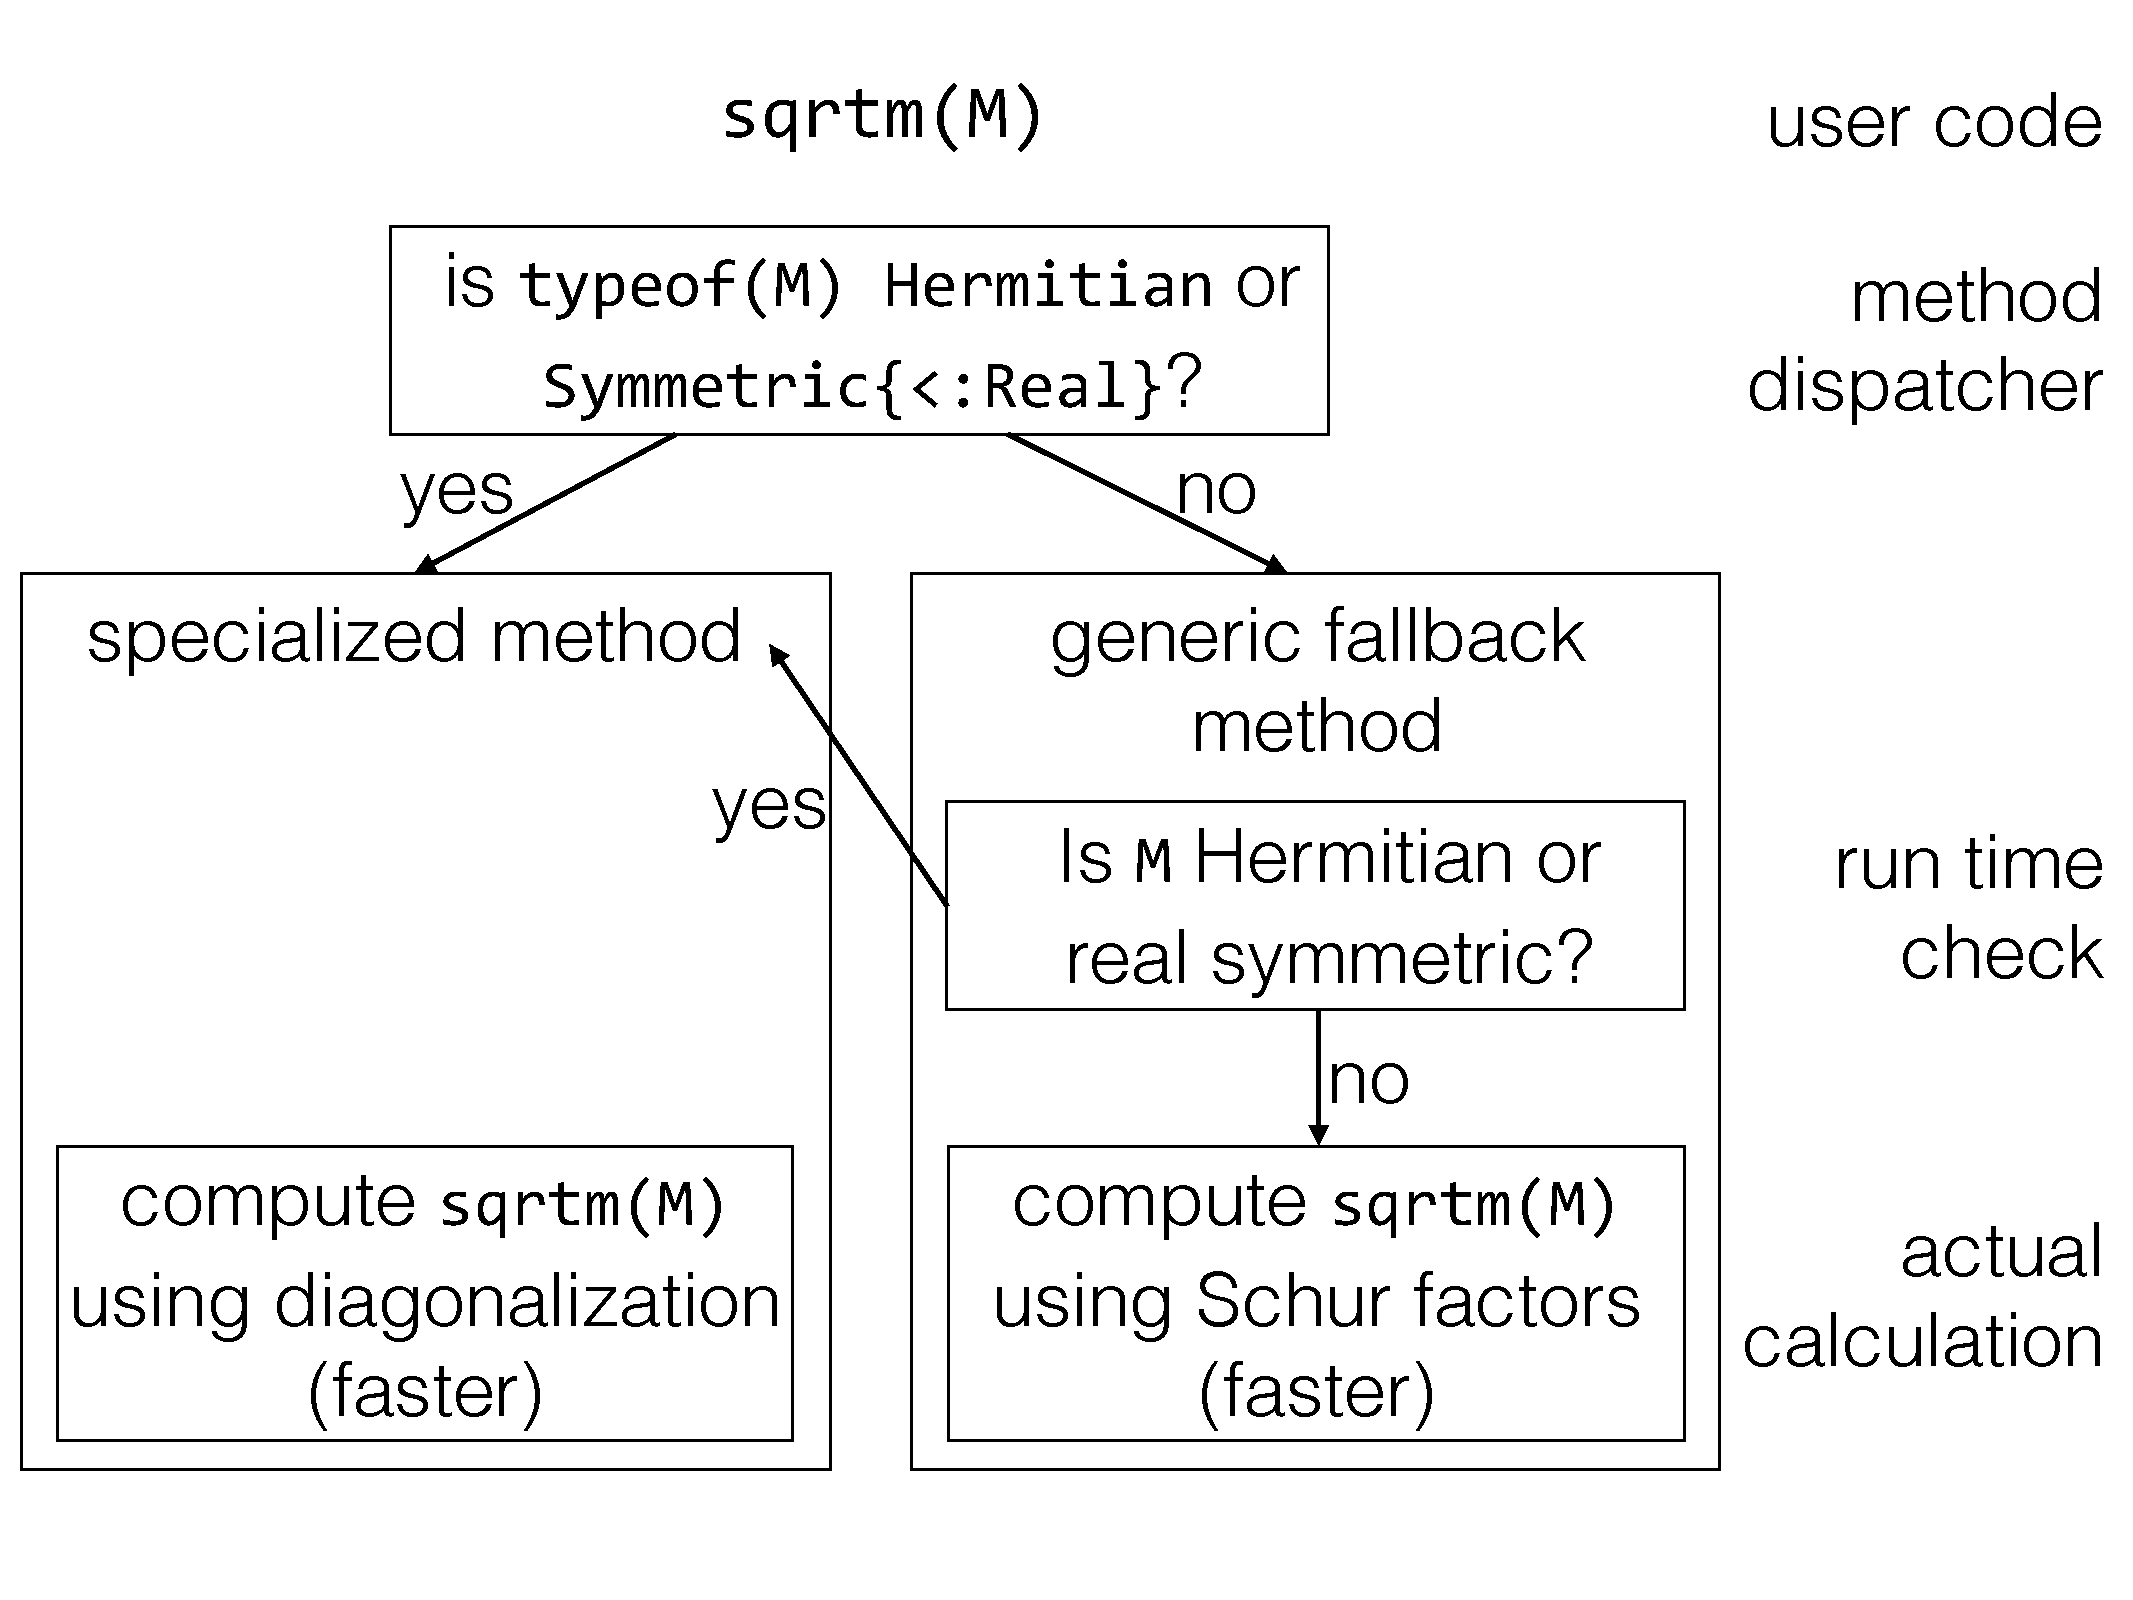
\includegraphics[width=\columnwidth]{fig-sqrtm}
	\caption{Dynamic dispatch and multimethods for the matrix square root
		function \texttt{sqrtm}, showing that the specialized algorithm
		can be run either from a static decision from the method
		dispatcher based on the input type, or a dynamic decision from
		a run--time check based on the value.}
	\label{fig:sqrtm}
\end{figure}


\subsection{Application: statistical library routines}

\paragraph{User interpretation of generic functions}
Generic functions express a common action or computation, which may in
practice be performed in many different ways depending on the inputs. For
example, one may wish to compute the mean of a given statistical distribution.
In Julia, the computation can be expressed simply as dispatch onto the method
\code{mean(D::Distribution)}, with a different method for \code{mean} being
defined for different \code{Distribution}s. In contrast, much scientific code
is written in languages that lack generic functions, resulting in users having
to keep track of a large family of very closely related functions which
together can be thought of as specialized mthods for a polymorphic function.
Table~\ref{statsfunctions} shows a family of closely related functions in the R
programming language and their Julia counterparts in the
\package{Distributions.jl} package. Julia provides a common functional interface
for each type of statistical distribution, with generic functions like
\code{pdf} to compute the probability density function, \code{cdf} for the
cumulative density function, \code{quantile} to compute quantiles, and
\code{rand} for sampling random variates. In contrast, each distribution in R
must have its own associated family of functions prefixed by \code{d},
\code{p}, \code{q} and \code{r} respectively, and the number of functions grows
by both the number of distributions and the number of desired computations on
them.

\code{pdf}
\begin{table}
{\tiny
\begin{tabular}{l || l | l | l | l}
  \textbf{\code{D}}                & \textbf{\code{pdf(D)}}    & \textbf{\code{cdf(D)}}    &
        \textbf{\code{quantile(D)}} & \textbf{\code{rand(D)}}  \\ \hline\hline
  \textbf{\code{Beta}}             & \code{dbeta}     & \code{pbeta}     & \code{qbeta}       & \code{rbeta}    \\
  \textbf{\code{Binomial}}         & \code{dbinom}    & \code{pbinom}    & \code{qbinom}      & \code{rbinom}   \\
  \textbf{\code{Cauchy}}           & \code{dcauchy}   & \code{pcauchy}   & \code{qcauchy}     & \code{rcauchy}  \\
  \textbf{\code{Chisq}}            & \code{dchisq}    & \code{pchisq}    & \code{qchisq}      & \code{rchisq}   \\
  \textbf{\code{Exponential}}      & \code{dexp}      & \code{pexp}      & \code{qexp}        & \code{rexp}     \\
  \textbf{\code{Fdist}}            & \code{df}        & \code{pf}        & \code{qf}          & \code{rf}       \\
  \textbf{\code{Gamma}}            & \code{dgamma}    & \code{pgamma}    & \code{qgamma}      & \code{rgamma}   \\
  \textbf{\code{Geometric}}        & \code{dgeom}     & \code{pgeom}     & \code{qgeom}       & \code{rgeom}    \\
  \textbf{\code{Hypergeometric}}   & \code{dhyper}    & \code{phyper}    & \code{qhyper}      & \code{rhyper}   \\
  \textbf{\code{LogNormal}}        & \code{dlnorm}    & \code{plnorm}    & \code{qlnorm}      & \code{rlnorm}   \\
  \textbf{\code{Multinomial}}      & \code{dmultinom} & \code{pmultinom} & \code{qmultinom}   & \code{rmultinom}\\
  \textbf{\code{NegativeBinomial}} & \code{dnbinom}   & \code{pnbinom}   & \code{qnbinom}     & \code{rnbinom}  \\
  \textbf{\code{Normal}}           & \code{dnorm}     & \code{pnorm}     & \code{qnorm}       & \code{rnorm}    \\
  \textbf{\code{Poisson}}          & \code{dpois}     & \code{ppois}     & \code{qpois}       & \code{rpois}    \\
  \textbf{\code{TDist}}            & \code{dt}        & \code{pt}        & \code{qt}          & \code{rt}       \\
  \textbf{\code{Uniform}}          & \code{dunif}     & \code{punif}     & \code{qunif}       & \code{runif}    \\
  \textbf{\code{Weibull}}          & \code{dweibull}  & \code{pweibull}  & \code{qweibull}    & \code{rweibull} \\
\end{tabular}
}
\label{statsfunctions}
\caption{List of common distributions in R v3.1.1\cite{rlang} and their
associated functions. Shown in bold are the equivalent Julia generic
functions and \code{Distribution} types provided by the Julia package
\package{Distributions.jl}, showing how the namespace
is simplified by generic functions and multiple dispatch.}
\end{table}

\TODO{show code examples}

\TODO{Other possible examples from Distributions.jl: QQ plots, posterior function}

\subsection{External dispatch with dynamic multimethods}

\paragraph{writemime example}
One thing you can do with dynamic multiple dispatch is external dispatch,
i.e.\ to be able to add new methods to an existing type rather than
specifying all the possible methods upfront. This is used to good effect
in Julia packages to extend functionality of the base library. For example,
the package \package{Color.jl} for manipulating color spaces extends the
\code{writemime} base function, which writes an object as a specified
MIME type\cite{mimerfc} to an I/O stream. \code{Color.jl} extends
\code{writemime} with new methods that draw color swatches.

\TODO{Here, we could put a figure showing writemime being called on a base
Julia object, writemime(::Color), and writemime(::VectorColor) objects.
Possibly take a screenshot in IJulia.}

\paragraph{External dispatch for package interaction}
External dispatch also facilitates interaction between Julia packages---
colors can be rendered using the \package{Cairo.jl} package,
which allows rendering to a Cairo backend~\cite{cairographics}.
When using Cairo to render an object in a given color, \code{Cairo.jl}
doesn't need to know anything about the underlying color space; it just
needs to call \code{convert} methods provided by \code{Color.jl}.
Julia's \code{convert} protocol is the ``narrow waist'' that allows
packages to allow using all kinds of color spaces naturally, without
needing to know anything specifically about them.

\paragraph{External dispatch is clunky in C++}
External dispatch can be performed in other languages like C++. However,
C++ only allows static external dispatch, which severely limits its utility.
Furthermore, external dispatch in C++ requires virtual methods and visitor
patterns\cite{designpatterns} to work around the absence of explicit support
for external dispatch.



\section{Performance}



\section{Related Work}

Dynamic dispatch is more general than static dispatch since it covers cases
which cannot be determined at compile time.  Common examples involve data
retrieval with a persistent storage, generating string representations for text
output or data serialization.\cite{Shields1998}

\paragraph{Exotypes in Lua}
Exotypes\cite{exotypes} provide to the Lua language\cite{lua} the analogue of
macros that generate staged functions\cite{stagedfunc} in Julia.

There are some notable differences, though:

Exotypes are programmed in Terra,\cite{terra} a separate layer on top of the
Lua host language, and method specialization must be explicitly invoked from
within Terra. The syntax incurred by having two language layers creates an
artificial distinction between built-in methods and user-defined methods that
doesn't exist in Julia.

Exotypes implement automatic broadcasting when there is a
\code{\_\_methodmissing} property defined. Julia does not use automatic
broadcasting to implement the Proxy design pattern.

Julia uses an eager approach to resolving circularity in method definitions.
Exotypes use lazy evaluation, although interestingly, earlier versions of Terra
also used eager evaluation~\cite{terra}.

\TODO{Multiple dispatch paradigm may obviate the need for exotypes in some uses and make exotypes more powerful in others}

In a multiple dispatch paradigm, the issues brought up in Lua/Terra in wanting
to being able to create types with an unbounded number of behaviors becomes
irrelevant. There is a separation of functions and objects in Julia that
obviates the need for lazily queried properties (although it may still be a
more efficient implementation choice).

\paragraph{Dylan}

Like Julia, dispatch is dynamic, except where the compiler has determined
(possibly with sealing optimizations) that it can be optimized into a static
dispatch.

Dylan is object-oriented in the style of Common Lisp, but unlike Common Lisp,
also integrates the object system into the language.

Dylan supports a limited form of parametric types, which are called limited
types.\cite{dylanman} This allows for some modicum of generic programming.

Dylan allows structural inheritance from concrete types by structural
inheritance, i.e.\ by adding fields on top of those in the parent type. In
Julia all concrete types are final: inheritance is only allowed from abstract
types which are essentially what OO researchers call traits. Dylan lacks
traits, which are a useful mechanism for expressing generic programs.

Julia's focus is not on objects, but rather on generic and functional
programming.

Dylan supports multiple inheritance, while Julia does not and instead resorts
to duck typing.

An extension for Dylan allows for gradual typing, allowing for type information
to be determined at compile time~\cite{Mehnert2010}.

\paragraph{Dynamically-typed $\lambda$-calculus}

Several extensions of typed $\lambda$-calculus have been developed to handle
dynamic types.

One flavor is described in \cite{Henglein1994}, where a special type tag
\code{Dyn} was introduced as a placeholder type that is dynamically coerced
into other types. %But this is not the kind of polymorphism that Julia has

Other examples of coercive polymorphic $\lambda$-calculi: the $F^\uparrow_C$
language of \cite{Vytiniotis2012,haskellkindtypes} used to describe the type
inference algorithm in GHC \cite{Weirich2011} contains type coercion
information that allows type errors to deferred to runtime
\cite{Vytiniotis2012} while preserving type-correctness. (This requires
so-called kind polymorphism, which allows for programs to reason about kinds.
\cite{haskellkindtypes})

%Attempt to explain Julia's polymorphism features

However, this describes coercive polymorphism \cite{Cardelli1985}, which
is arguably not true polymorphism in the sense that it is not
universal~\cite{Strachey1967,Strachey2000}. In contrast, Julia supports two
distinct mechanisms for universal polymorphism, namely subtyping (a special
case of inclusion polymorphism), and parametric polymorphism.

Julia is not a true polymorphic system in the sense of \cite{Cardelli1985},
where code is generated only once for every generic procedure. Julia generates
a variety of specialized methods and so are more in the send of Ada-style
generic procedures which are abbreviations for sets of monomorphic procedures.

%Staged functions, dynamic λ-calculus, gradual typing... all seem to be closely related aspects of the same thing: it is often advantageous to split the determination of type information between compile time and runtime.

\paragraph{Haskell}

The main strategy in Haskell to deal with types that are not statically
decidable is to use staged type inference.~\cite{Shields1998}

\TODO{
Dynamic typing in polymorphic languages
M. Abadi, L. Cardelli, B. Pierce and D. Rémy Journal of Functional Programming / Volume 5 / Issue 01 / January 1995, pp 111 - 130 DOI: 10.1017/S095679680000126X
}



\section{Implementation challenges}

\subsection{Type stability}
New users migrating from other dynamic languages like MATLAB, Python and R are
often surprised that direct, line--for--line translations to Julia do not
achieve claimed C--like performance. Empirical reports~\cite{julia-users}
indicate that such users are unfamiliar with reasoning about types. One common
pitfall is \textbf{type instability}, which is exemplified in the following
code:

\begin{lstlisting}
function f()
   x = 0
   for y=1.0:1000000.0
      x += y
   end
end
\end{lstlisting}
%
This seemingly innocuous routine runs slowly because \verb|x| is initialized to
\verb|0| which is of type \verb|Int|, but accumulates floating point values
\verb|y| of type \verb|Float64| and so within the inner loop undergoes type
promotion to \verb|promote_type(Int,Float64)| \verb|== Float64|. The data flow
analysis thus cannot deduce that \verb|x| is a concrete type, but only that it
is of type \verb|Union(Int,| \verb|Float64)|. Thus the generated LLVM code must
call back to the Julia runtime to determine the value's actual type, and hence
boxes the value \verb|x|. As a result, \verb|x| cannot be mapped onto an LLVM
register, but must instead be heap allocated.

Another class of type instabilities results from the subtle interaction of
parametric invariance, the use of non-leaf type parameters and type promotion.
For example, the parametric type \verb|Complex{FloatingPoint}| is
type--unstable under addition (\verb|+|):

\begin{lstlisting}
function g()
    x = Complex{FloatingPoint}(1.0, 2.0f0) #(Float64, Float32)
    x + x #inferred type is Complex
end
\end{lstlisting}
%
Calling \verb|g()| returns a value of type \verb|Complex{Float64}| because the
\verb|+| method called uses the external constructor

\begin{lstlisting}
Complex(x::Real, y::Real) = Complex(promote(x,y)...)
\end{lstlisting}
%
which promotes the real and imaginary components to a common supertype (in this
case, \verb|Float64|). Since type parameters are invariant, the resulting type
is neither a subtype nor a supertype of the original type.

Most static languages like C require users to explicitly reason about type
instabilities (e.g.\ by requiring type casts); most dynamic languages allow
type--unstable code, but at the price of degraded performance. Julia allows
users to inspect the results of type inference and modify their codes to
improve performance by sharpening type annotations on variables, using language
constructs described in Section~\ref{sec:inference}.


\subsection{(Data) vectorization}

New Julia users are also often surprised that vectorized expressions in Julia
can be slower than their devectorized counterparts. Consider the function

\begin{lstlisting}
h1(x) = sin(x) + im*cos(x)
\end{lstlisting}
%
For scalar numbers \verb|x| of type \verb|Float64|, \verb|h1| constructs a
complex number of type \verb|Complex{Float64}|. However, \verb|h1| also accepts
arrays of type \verb|Array{Float64, N}| (where $N$ is the rank), returning a
corresponding array \verb|Array{Complex| \verb|{Float64}, N}|.

In other dynamic languages, vectorization is an accepted mantra for
performance~\cite{matlabuserguide,Langtangen2008}, as the vectorized functions often wrap
kernels written in a low--level language that deliver performance over
functionally equivalent devectorized code which use slow, directly interpreted
scalar loops~\cite{Seljebotn2009,Walt2011}. Users have therefore learned that
vectorized functions provide speed, and will sometimes go to great lengths to
contort their computations into vectorized form to speed up their code, even if
the computation cannot be expressed conveniently or naturally in vectorized
form. Furthermore, vectorization still incurs significant overhead,
particularly in the unwanted allocation of array temporaries. In this example,
\verb|h1| constructs three temporary arrays on top of the new array needed to
contain the answer, namely the arrays \verb|A|, \verb|B| and \verb|C| in the
equivalent code: 

\begin{lstlisting}
function h2(x)
    A = sin(x) #Apply sin to each element of x, etc.
    B = cos(x)
    C = im * B
    D = A + C
    return D
end
\end{lstlisting}
%
In contrast, the devectorized version of the same code

\begin{lstlisting}
function h3(x)
    z = similar(x) #Construct array with same shape as x
    for (i, y) in enumerate(x)
        z[i] = sin(y) + im*cos(y)
    end
end
\end{lstlisting}
%
computes the same result but avoids allocating temporary arrays and their
concomitant overhead costs for heap allocation, memory access and garbage
collection. Thus devectorized code is preferred in Julia as scalar loops are
fast with minimal overhead~\cite{Bezanson2014b}. 


\subsection{Vectorization and higher--order functions}

Another more subtle issue with vectorized functions is their limited
extensibility and composability. Implementations can only bless some
functions to be vectorized; vectorized functions which wrap external low--level
kernels lack code reuse and cannot be extended easily. In contrast, the Julia
standard library implements vectorized functions consistently using using code
generated by the macros \verb|@vectorize_1arg|, \verb|@vectorize_2arg| etc.

The composability problem is more subtle. The generic function \verb|h1| has
methods with function types

\begin{itemize}
	\item \verb|Float64| $\rightarrow$ \verb|Complex{Float64}|,
	\item \verb|Vector{Float64}| $\rightarrow$ \verb|Vector{Complex{Float64}}|,
\end{itemize}
%
and others, and writing a function \verb|i(x)| that composes properly with
\verb|h1| must account for all possible outputs of the latter, be they scalars
or arrays. Thus \verb|i(x)| must also be vectorized, but the dynamic nature of
Julia precludes any restrictions on the methods that must be defined for
\verb|i|, placing the burden of correct implementation on users and library
writers.

The example of \verb|h1| suggests that what users really want is not vectorized
functions, but rather convenient syntax for vectorized \textit{expressions}.
The \package{Devectorize.jl} package uses code generation techniques to marry
the convenient syntax for vectorized functions with the speed of devectorized
code with explicit loops. The restructuring for vectorization is often
unnatural, and at times not possible. Alternatively, a more general approach is
to use higher order functions like \verb|map| to compute an entire vectorized
expression, like so:

\begin{lstlisting}
h3(x) = map(_ -> sin(_) + im*cos(_), x)
\end{lstlisting}
%
\verb|map| provides an elegant solution to mapping a computation over a
collection of input data. However, implementing \verb|map| efficiently in Julia
touches upon all the aspects of the type system, generic function system,
dispatch, and type inference that have been discussed above:

\begin{enumerate}

	\item The output type of \verb|f| must be an \verb|Array{T}| with
	element type \verb|T| wide enough to describe all the possible output
	elements. \verb|T = Any| is the widest possible array, but provides no
	information about the mutability of each element. Consequently the
	array must be represented in memory with pointers to boxed elements. In
	contrast, being able to infer a concrete immutable element type like
	\verb|T = Float64| allows the indirection to array elements and the
	overhead of tagging to be eliminated, allowing the resulting array data
	to stored contiguously like a C or Fortran array.

	\item To know the output type of \verb|f(y)| for some element \verb|y|
	of \verb|x|, the type of \verb|y| must be known so that the actual
	method being dispatched for the generic function \verb|f| can be looked
	up in the dispatch table. This means that the data \verb|x| must be
	fully typed within the type environment where \verb|map| is invoked.
	Furthermore the type environment must yield enough information about
	\verb|y| so that the method dispatcher is able to pick out a
	specialized method over the generic fall--back for \verb|f|.

	\item Since Julia lacks true function types, the output type of
	\verb|f(y)| must be inferred from data flow analysis, and the inferred
	type must be sufficiently sharp to determine the type of the output of
	\verb|map|.

	\item For performance, the scalar operation \verb|f(y)| must be
	inlined, and hence the inlining code transformation pass must deem the
	inlining to be viable.

	\item Implementing \verb|map| over an arbitrary iterable \verb|x| is
	harder than implementing vectorized functions, since the former lacks
	the guarantee provided by \verb|Array| inputs types that every element
	has the same type. In the worst case, the method dispatcher must be
	called for each element \verb|y| just to find out which method is
	dispatched for \verb|f(y)|.

\end{enumerate}

The implementation of \verb|map| hence speaks to the conflicting demands of
flexibility and performance that underlie the design tradeoffs built into
Julia's types, generic functions and type inference algorithms. The current
implementation leverages empirical evidence that most applications use
homogeneous arrays of concrete types, and most other applications have
heterogeneity that be detected early on~\cite{Bolz2013}. Hence, \verb|map|
optimistically assumes an element type based on the output returned from the
first element, and makes further copies into increasingly wider arrays as
necessary if a later return type is wider than the current element type. The
number of such copies made is bounded by the maximal height of the type
lattice, and the aggressive method specialization in Julia's compiler can emit
specialized code which optimize away branch checks for widening in cases where
the input type is completely known, e.g.\ when the input is an \verb|Array|
with some concrete element type, and thus avoid the cost of conditional
branches.

Julia as a language is still evolving, and there is room for further
improvements to the compiler, such as additional static analyses for peephole
optimizations, constant propagation, and backward data flow type inference.
Nevertheless, the current type system, generic function system with
multimethods and type inference with aggressive method specialization afford
rich semantics which are useful for technical computing applications.
Furthermore, the design and interaction between these language components allow
users to design their own Pareto--optimal tradeoffs between performant
specialization and flexible generality within a single programming language.

\acks{We thank the many Julia users and developers for their contributions to
the Julia language.}

%The authors gratefully acknowledge support from the MIT Deshpande center for
%technical innovation, the Intel Technology Science Center for Big Data, the
%DARPA XDATA program, the Singapore--MIT Alliance, NSF Awards CCF-0832997 and
%DMS-1016125, VMWare Research, a DOE grant with Dr. Andrew Gelman of Columbia
%University for petascale hierarchical modeling, a Citibank grant for High
%Performance Banking Data Analysis, and the Levine Fellowship.}

\listoftodos %TODO remove from final submission

\bibliographystyle{abbrvnat}
\bibliography{pldi2015,websites}

\end{document}
